%! Author = vladislav.yaroshchuk
%! Date = 10/10/2021

\pagebreak


\section{Соотнесение ключевых понятий между собой, построение тезауруса.}

Информационно-поисковый язык (ИПЯ) — формализованный искусственный язык, предназначенный для
индексирования документов, информационных запросов и описания фактов с целью последующего хранения
и поиска (ГОСТ 7.74-96).


Информационно-поисковый тезаурус (ИПТ) — нормативный словарь дескрипторного ИПЯ с зафиксированными
в нем парадигматическими отношениями лексических единиц (ГОСТ 7.74-96).
В отличие от толкового словаря, тезаурус позволяет выявить смысл не только с помощью определения,
но и посредством соотнесения слова с другими понятиями и их группами.
Задачей этапа является определение соотношений между понятиями, выделенными на предыдущем этапе.

\begin{figure}[ht]
    \begin{center}
        \scalebox{0.4}{
            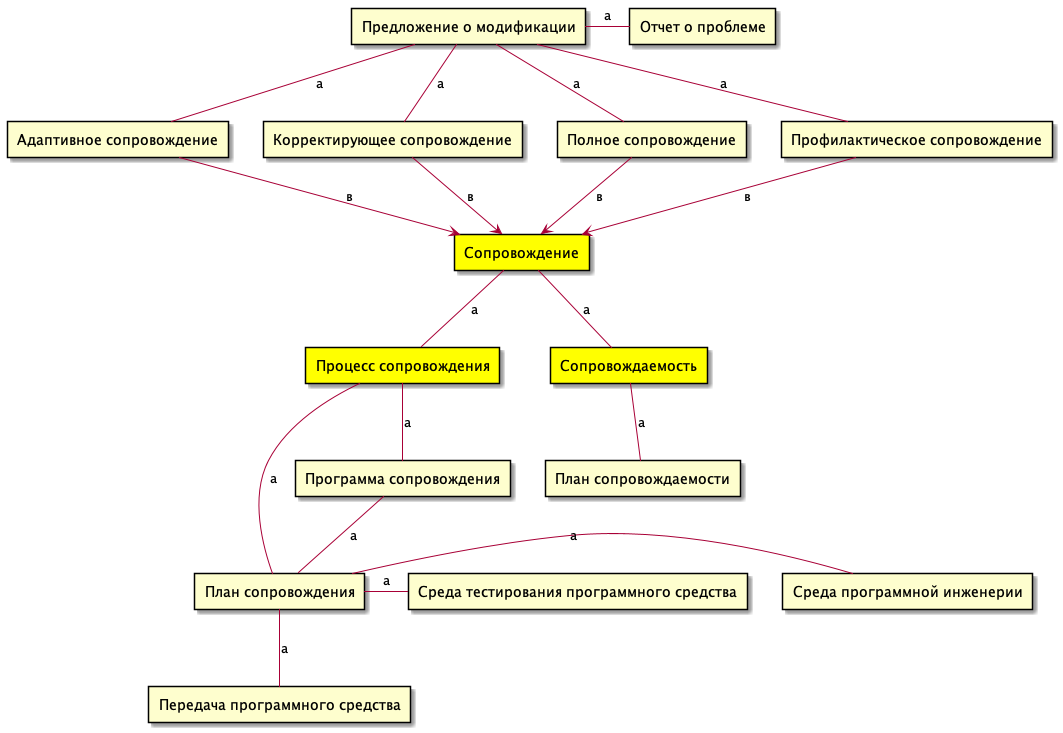
\includegraphics{images/thesaurus}
        }
    \end {center}\label{fig:figure}
\end {figure}
